\section{Design}\label{sec:design}

In this section, we present our system design of \sysname and discuss technical details we apply in \sysname.

%\subsection{Motivation} 
%
%Fuzzing has been proved to be an effective technique to find software bugs. However, although this technique has been widely used in software security for years, even today we still rarely see its application in the field of IoT security. 
%
%%[Why Fuzzing]?
%Previous solutions for security analysis in IoT device can be categorized based on different analysis approaches they take. For example, Costin et al.~\cite{costin2014large} leverage on static analysis techniques to automatically unpack a large number of firmwares and then search for specific patterns to find existing security flaws in them. On the contrary, Chen et al.~\cite{chen2016towards} design a dynamic analysis system for Linux-based IoT device's firmware. It takes an emulator-based approach to identify software vulnerabilities by performing large scale automated black-box testing with various existing exploits. While these solutions are efficient and scalable, they either suffer from accuracy issues due to inherited limitations of static analysis or lack compatibility with various types of IoT devices. \hl{More importantly, all these previous research focus on identifying existing software security flaws.}
%
%Consequently, our goal is to provide efficient and comprehensive security analysis in Linux-based IoT devices and search for unknown security bugs by adopting fuzzing techniques in binary programs. 

%\subsection{Challenges}
%
%As mentioned earlier, fuzzing on IoT devices poses the following major challenges in comparison with fuzzing on x86 platforms.
%
%\begin{enumerate}
%\item \textbf{Limited Resources.} In comparison with x86 platform, IoT devices often have very limited resource in terms of CPU, memory and storage. Generally, it requires additional migration and optimization work to integrate a fuzzer with the origin operating system. Consequently, there must be a trade-off between accuracy and efficiency when it comes to the system design, otherwise the fuzzing will be infeasible. 
%
%\item \textbf{No source code available.} Commercial-off-the-shelf (COTS) IoT devices are usually installed with many proprietary software. Generally, source code and documentation of such software are not available, which makes it difficult to apply coverage-based grey-box~\cite{} fuzzing techniques in these software. 
%
%\item \textbf{No shell access.} For security concerns, shell access from network is strictly forbidden in most COTS IoT devices, which makes it difficult to deploy fuzzer in the target IoT devices.
%
%\item \textbf{Various CPU architecture, instructions and tool-chains.} Unlike x86 platform, various types of CPUs with different architectures and instructions are used in the domain of IoT devices. Such differences bring significant challenges to binary-level program analysis and instrumentation. Besides there is also a rich diversity of tool-chains that developed for different CPU architecture, which inevitably increases the difficulties of fuzzing on IoT devices. 
%\end{enumerate}


\subsection{Approach Overview}

We design and implement {\sysname}, a fast, lightweight and easy deployable coverage-based fuzzing framework for binary programs on Linux-based IoT device. The primary goal of {\sysname} is to provide practical solution for security researchers to automatically analyze software on IoT devices where source code is usually unavailable.

Generally, there are several different approaches to implement coverage-based fuzzing on binary programs. The first approach that comes mind is to use virtual machine emulation. As mentioned in Section~\ref{sec:background}, AFL leverages QEMU to hook instructions at each branch point in order to track execution of the target binary program. In this way, it achieves runtime instrumentation without modifying the target binary program. While this approach can provide the most accurate branch coverage information, it is too expensive to apply in IoT devices.

The next approach we can easily think of is assembly-level instrumentation which leverage on a disassembler as well as an assembler. Compared with the original binary program, assembly-level instrumentation only produces a small runtime overhead and all data references and function pointer access can be easily resolved by assembler after the instrumentation. However, this approach requires very high accuracy for both disassembler and assembler, which could be very challenging, especially for large complex binary programs.

%which pose 

%Unfortunately, in practice there is no tool available that meets such requirement, especially on large complex binary programs.

%However, in practice there is no disassembler available which can meet that precision requirement

%The advantages of this approach are that the instrumentation overhead is small in comparison with the original program and all data references and function pointer accesses can be easily resolved during the instrumentation. 

%However, such advantages only hold when the disassembler can precisely recognize all of the instructions and data within the original binary program.
%Unfortunately, in practice there is no disassembler available which can meet that precision requirement especially on large complex binary programs. As a result, disassemblers are usually used as auxiliary tools in reverse engineering tasks and therefore assembly-level instrumentation is also infeasible.

{\bf Our Approach: Binary-level instrumentation.}
Considering the infeasibility of the above two approaches, we choose binary-level instrumentation in our design. That means to statically instrument the target binary program with binary code that tracks coverage information during the fuzzing process. In our approach, instrumented code is injected at each branch point to track the execution of each basic block. So, we first identify all basic blocks in the binary program, then inject binary code at the beginning of each basic block. In this way, our approach maintains all the code and data structures in the original program and therefore avoid breaking its code logic.

%Although some existing tools (e.g. afl~\cite{aflwhitepaper}) have already provide capability to fuzz binary programs on x86 platform by adopting virtualization technology, there are still two major challenges to fuzz binary programs in IoT device's firmware in Virtual Machine: 


%\begin{enumerate}
	%\item Unlike many x86 platforms, most of IoT devices often have very limited resources, so VM-based solution is too expensive and in most cases is not even applicable on IoT devices.
	%\item Binary programs in IoT device's firmware often require specific runtime environment or even additional hardware support (e.g. NVRAM), which are extremely challenging to emulate in a VM.
%\end{enumerate}


%As a consequence, instead of running the target binary program inside a VM, we take a more efficient approach by adopting binary level instrumentation techniques in our system design. 

Generally, our approach has the following advantages: 1) It is lightweight and achieves almost the equivalent efficiency with source-code-level instrumentation~(See Section~\ref{sec:eval:performance}). 2) It is compatible with many IoT devices because it fuzzes the target program on the original device and therefore does not require migration work such as environment configuration and dependence installation. 3) The accuracy of instrumentation will not affect the correctness of the target program execution. It will only affect the coverage information that are collected during the execution of the target program.



\begin{figure*}[htbp]
\centering 
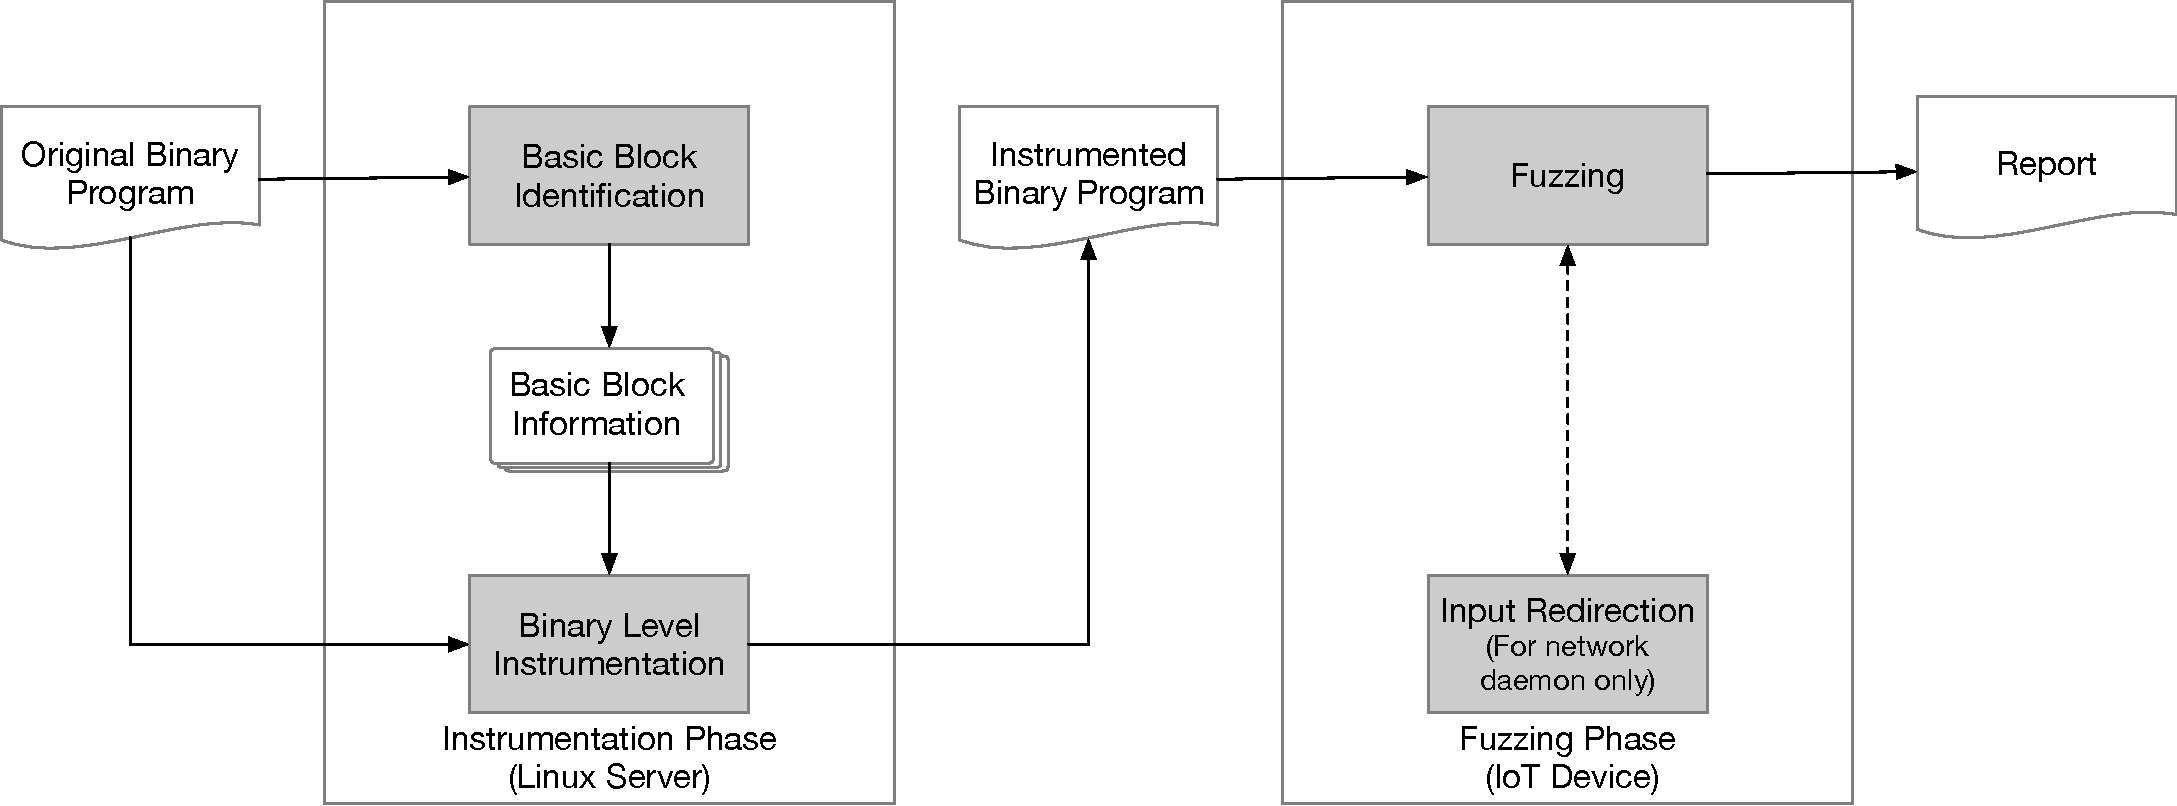
\includegraphics[width=0.9\textwidth]{arch}
\caption{ Overview of \sysname.}
\label{figs:arch}
\end{figure*}

The system overview of {\sysname} is illustrated in Figure~\ref{figs:arch}. Specifically, there are two phases in the workflow of \sysname: \textbf{instrumentation phase} and \textbf{fuzzing phase}.

In the instrumentation phase, we develop an elf-patcher and it first takes a binary program as an input, and then identifies and locates all of its basic blocks by disassembling and analyzing the binary code. Next, a small code stub for recording branch coverage is automatically instrumented into the beginning of each basic block that the elf-patcher identified. Finally, a code stub for initialization and communication with the fuzzer is automatically registered as an initialization entry of the target program. To guarantee the efficiency, all steps in the instrumentation phase are performed outside the target IoT devices. 

In the fuzzing phase, both the instrumented program and the fuzzer are deployed on the original device before an instrumentation-guided coverage-based fuzzing is performed and all the fuzzing results are recorded. Besides, IoT devices usually contains many network daemon software (e.g. a web server), so we also design and implement an input redirection framework for fuzzing on network daemons.

Overall, \sysname provides two major features: binary-level instrumentation and network input redirection. We will go through the technique details of these features in following subsections.


%[Why binary program fuzzing]?

%disassembling suffers from accuracy issues...
%Why we patch binary

% 1. The prevalence of linux-based IoT device
% 2. lack of source code 
% 3. 

%[Why coverage-based grey-box]?

%[emulator vs devices]
% 1. The limitation of emulator-based approach kernel module, 
% 2. The 




\subsection{Basic Block Identification}


The basic idea of instrumentation-guided coverage-based fuzzing is to improve execution coverage by monitoring each execution path of the target program for different inputs. To this end, each basic block of the target binary program needs to be identified with good accuracy before instrumentation. A basic block is a straight-line code sequence with no branches in except the entry and no branches out except at the exit~\cite{hennessy2011computer}. Once the execution of the target program enters a specific basic block, all code inside this basic block must be sequentially executed. 

%To ensure the accuracy of tracking execution path, a code stub which is responsible to communicate with the fuzzer needs to be instrumented into each basic block of the target program.

%Before instrumentation, it is very important to identify all the basic blocks inside the target program. %To this end, 

As illustrated in Figure~\ref{figs:arch} \sysname first leverages a static analyzer to perform reverse engineer on the target binary program including generating a hierarchical call graph and extracting a list of functions. Then for each function, \sysname checks if it can be triggered from entry point of the program by performing a backward search on the call graph. Such check eliminates those unreachable basic blocks from the results and therefore improves the efficiency of \sysname. Next, \sysname marks all reachable functions, and for each function it again leverages the static analyzer to search for all basic blocks within this function. Finally, \sysname merges the searching result, eliminates duplicated basic blocks and logs all the information (e.g. type of instruction set, base address of the basic block, size of the basic block, etc.) of each basic block for later use.

\subsection{Binary-level Instrumentation}\label{sec:design:inst}


\begin{figure}[htbp]
\centering 
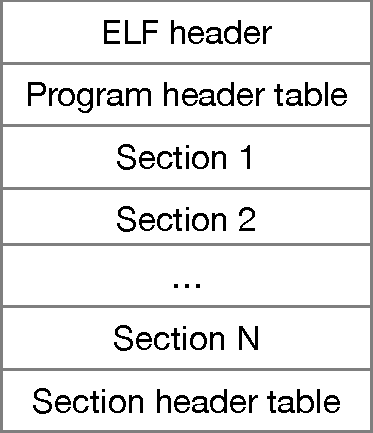
\includegraphics[width=0.2\textwidth]{elf}
\caption{Executable and Linkable Format~(ELF) File Structure.}
\label{figs:elf}
\end{figure}


\sysname targets at Executable and Linkable Format ~(ELF)~\cite{elf} binary program which is used in most Unix-like operating system. The binary-level Instrumentation that perform by \sysname is pure static and therefore only takes the target program and its basic block information as a input. 

The structure of a typical ELF file is described in Figure~\ref{figs:elf}. $ELF\ Header$ contains the basic information of the file, such as instruction set and architecture. Besides, $ELF\ Header$ also stores the position and size for both $Program\ Header\ Table$ and $Section\ Header\ Table$. $Program\ Header\ Table$ defines run-time information for the binary program. For example, $PT\_LOAD$ entries specific the mapping between sections and memory segments, $PT\_DYNAMIC$ entry specifics the position and size for $.dynamic$ section. $Section\ Header\ Table$ specifies position and size for each section within the ELF file. Such information is useful during the linking process. $Sections$ are segments where code and data are actually stored in an ELF file. There are various types of sections that defined in an ELF file, such as $.text$ section, $.data$ section, etc. Generally, $Program\ Header\ Table$ is not necessary for ELFs during linking while $Section\ Header\ Table$ is omittable for ELFs during run-time. However, most of compilers tend to keep both tables at the same time.

Our basic idea of instrumentation is to add code stub into each basic block without breaking the code logic of the original program. However, in a compiled ELF binary program, there is no space for the instrumented code in the original sections because the addresses for all the instructions and data have already been calculated by the compiler and moving such instructions or data at binary-level will likely disrupt the execution of the original program. Consequently, our solution makes extra space for instrumented code by adding new sections at the end of the ELF binary program.

As shown in Figure~\ref{figs:instrumentation}, for each basic block, we replace its first instruction $inst\_A$ with a branch instruction that redirects the program counter (PC) to a newly added section where our instrumented code is executed. Then, the replaced instruction $inst\_A$ is moved after the instrumented code. Finally, another branch instruction is added at the end of the new section to redirect PC back to the next instruction $inst\_B$ in the original section. Generally, our solution performs the following three steps for binary instrumentation:

\begin{figure}[htbp]
\centering 
\begin{subfigure}[b]{0.20\textwidth}
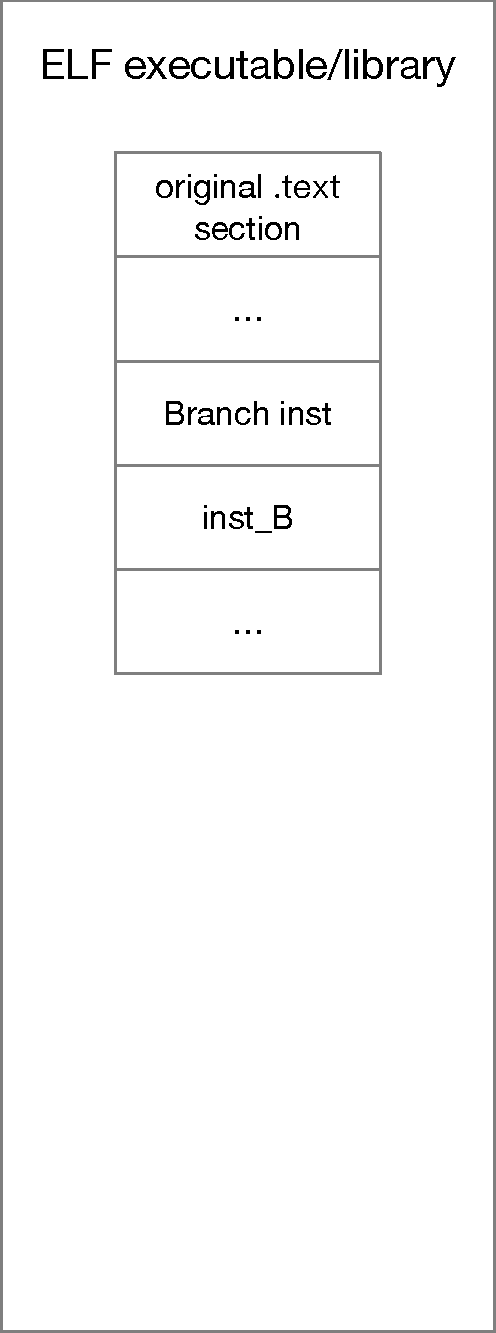
\includegraphics[width=\textwidth]{instrumentation_a}
\caption{Original ELF file}
\end{subfigure}
\hspace{+8pt}
\begin{subfigure}[b]{0.20\textwidth}
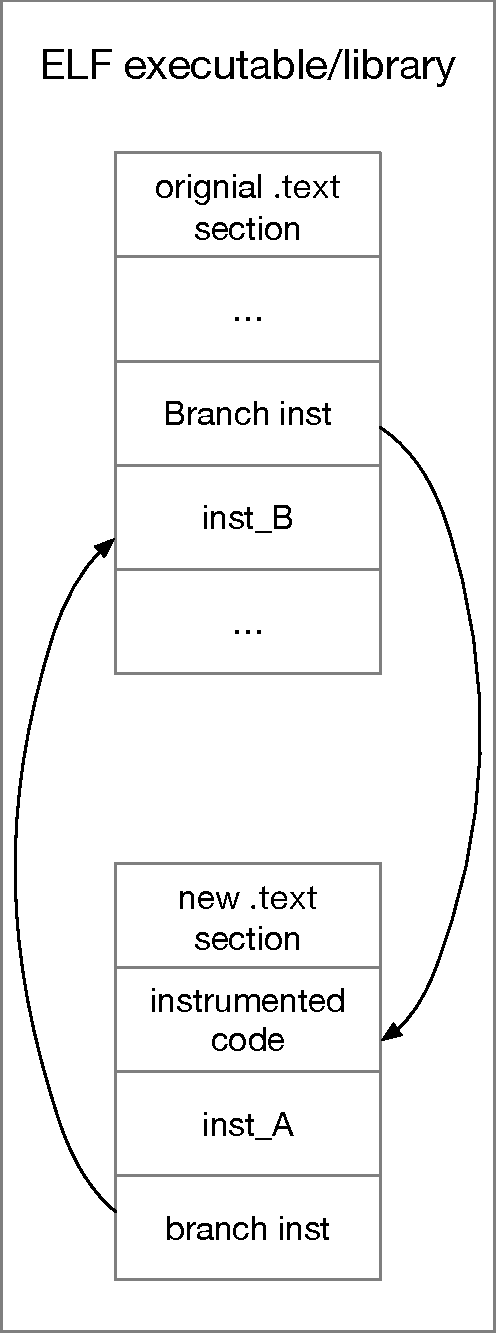
\includegraphics[width=\textwidth]{instrumentation_b}
\caption{Instrumented ELF file}
\end{subfigure}
\caption{Binary-level Instrumentation.}
\label{figs:instrumentation}
\end{figure}

\begin{enumerate}
	\item Adding new sections for instrumented code and data and updating $Section\ header\ table$ for these new sections.
	\item Adding new $PT\_LOAD$ entry in $Program\ header$ $table$ to make sure all newly added data is loaded into the memory during execution.
	\item Replacing the original instructions and adding instrumented instructions and data.
\end{enumerate}

\vspace{5pt} 
\subsubsection{\bf{Adding New Sections}}
The approach we take to add new sections in ELF binary program is quite straightforward. For new data section, we first calculate the length of the inserted data and determines the address and size of the new section. Then we add these sections directly at the end of the last section in the original program. Meanwhile, for each new data section, we will add a new entry in $Section\ header\ table$ to specify its address, offset and size. Moreover, since we expand the size of $Section\ header\ table$ which therefore increases the size of the ELF file, the ELF header also needs to be modified accordingly.

However, things are getting a little bit complicated when adding new code sections. Our code instrumentation relies on the assembler to generate new instructions. Without the size information of the newly added code section, the assembler has no idea of the section layout and relative offset from the original instructions to the inserted code stub, therefore the assembler cannot generate correct instructions for the new stub. However, the size of the new code section depends on the length of the instrumented instructions, which can only be determined by the assembler. In other words, there is a deadlock.

To solve this deadlock, our solution is to take two assemble passes. In the first pass, we assume the address for the original instructions with which the assembler is able to calculate the length of the instrumented instructions. In this way, the size of the new code section is determined and can be used in the second pass for code instrumentation.

%To solve this deadlock, our solution is to let the assembler take two passes. In the pass, we first assume the addresses for the original instructions with which the assembler is able to calculate the length of the instrumented instructions. In this way, the size of the new code section is determined and can be used in the second pass for code instrumentation. \\
\vspace{5pt} 
\subsubsection{\bf{Updating Program Header Table}}
Sections are static information in an ELF binary program. Therefore the instrumented data and instructions will not be loaded into memory by simply adding new sections to the original ELF program. We need to add $PT\_LOAD$ entries for all new sections to specify the access permission for each segment of data and the memory address where it should be loaded to.

Unlike $Section\ header\ table$ which is located at the end of the ELF file~(shown in Figure~\ref{figs:elf}), expanding $Program\ header\ table$ will inevitably erase sections that comes after it. To avoid the such conflict, we come up with two solutions: 1. Moving $Program\ header\ table$ behind all sections. 2. Moving those sections that come after $Program\ header\ table$ backwards. Unfortunately, in practice the first solution is infeasible because Linux kernel assumes that $Program\ header\ table$ comes immediately after ELF header. In other words, it will result in a failure when running the instrumented program if we moved the $Program\ header\ table$ elsewhere. We therefore adopt the second solution. We first analyze a large number of ELF binaries that we collected from dozens of IoT device firmwares. The statistics show that only certain types of section~(Table~\ref{table:elfsecs}) appears immediately after $Program\ header\ table$. All these types of sections have their location information stored in $Program\ header\ table$ or $.dynamic$ section, so they can be relocated by simply modifying the pointers accordingly. 
\begin{table}
\center
\begin{tabular}{|l|l|}
\hline 
Section & Description \\ 
\hline 
.interp & Absolute path of the loader \\ 
\hline 
.note. & Additional information about the ELF \\ 
\hline 
.hash & Symbol hash table \\ 
\hline 
.gnu.hash & GNU style symbol hash table \\ 
\hline 
.dynsym & Symbol table \\ 
\hline 
.dynstr & Strings used by .dynsym \\ 
\hline 
\end{tabular}
\caption{Types of sections that may appears after $Program\ header\ table$ in an ELF binary program.}
\label{table:elfsecs}
\end{table}

After moving all these sections, we can easily expand the $Program$ $header\ table$ by adding new entries without any conflict. For each type of the sections that we added or moved, we add a corresponding $PT\_LOAD$ entry to $Program\ header\ table$. Besides, newly added sections are granted with one of the three access permission: $READ\_ONLY$, $READ\_WRITE$ and $READ\_EXECUTE$, which is reflected in their $PT\_LOAD$ entries.
\vspace{5pt} 
\subsubsection{\bf{Wrapping Original Instruction}}\label{sec:design:wrap}

As shown in Figure~\ref{figs:instrumentation}, our code instrumentation first replaces the first instruction $inst\_A$ in each basic block of the target program with a branch instruction and thus redirect the execution to our newly added .text section. Instrumented code, the replaced $inst\_A$ and another branch instruction are then sequentially inserted into the new section.

Binary level instrumentation could be very tricky for CISC architecture~(e.g. x86), where instructions usually have variable lengths. So replacing one instruction with another may overwrite the subsequent instructions. Fortunately, most IoT devices are built upon RISC architecture~(e.g. ARM, MIPS, etc.) with fixed instruction length. As a result, $inst\_A$ can be easily replaced with a branch instruction without touching the instruction that comes after it. 

One major challenge to apply our code instrumentation is that we need to guarantee the successful execution of the original $inst\_A$~(See Figure~\ref{figs:instrumentation}) in the new location. To this end, our instrumented code maintains the values in all registers or memory addresses that are used in the original program. Specifically, our instrumented code first backs up all registers before using them and recovers those values at the end. For memory addresses, our instrumented code only writes to unused addresses below the current stack pointer to avoid potential conflicts. 

Besides, some instructions use the value of program counter~(PC). Since the value of PC varies at different position in a program, moving these PC-related instructions to new locations~(e.g. $inst\_A$ in Figure~\ref{figs:instrumentation}) may disrupt the executions of the origin program and thus result in errors. To eliminate such effect caused by PC, in our approach we first divide all instructions into the following five types based on their different relationship with PC. Then for each type, we provide a different wrap solution to the original instruction.

\begin{itemize}

\item \textbf{T1: PC-independent instruction.} These are instructions that are completely independent from the value of PC. In other words, they are not related to any computation or memory access based on the value of PC.

\item \textbf{T2: PC-dependent branch instruction.} Some branch instructions (e.g. $b$ in ARM instruction set) depend on the value of PC to determine the destination address. An offset which is relative to PC can be used as an operand to indicate the destination address.
 
\item \textbf{T3: PC read-only instruction.} These are the instructions that take the value of PC as one of their source operands, and then either assign it to another register or load a value from the memory with a relative offset to current PC.

\item \textbf{T4: PC read-only instruction with stack operation.} These instructions take the value of PC as their source operand which works just like T3 except they also involve in stack operation.

\item \textbf{T5: PC read-write instruction.} These instructions involve in both read and write operations that are related to PC.

\end{itemize}

\noindent{\bf Wrap Solution.} For each type of instruction~(T1 to T5), our approach provides a wrap solution~(S1 to S5) to eliminate the effect caused by different PC values at new positions in the target program.

\begin{itemize}

\item \textbf{S1. }~For PC-independent instruction~(T1), it will not affect their execution by moving it to a new location. As a result, no specific wrap solution is needed other than simple branch back.

\item \textbf{S2. }~For PC-dependent branch instruction~(T2), although its destination address is determined based on the value of PC, the destination address can be easily obtained by disassembling this branch instruction in the original program. In this way, the branch instruction becomes PC-independent and therefore does not require any specific wrap solution either.

\item \textbf{S3. }~For PC read-only instruction~(T3), we first find a unused register as $pivot$ and save its original value to stack. Secondly we get the value of PC at the original position of the target instruction~(e.g. $Inst\_A$ in Figure~\ref{figs:instrumentation}(a)) by using a disassembler and save it to $pivot$. Then we replace each occurrence of PC register with $pivot$ in the target instruction at new position~(e.g. $Inst\_A$ in Figure~\ref{figs:instrumentation}(b)). In the end, the value of $pivot$ register is recovered from stack after the execution of the target instruction at new position.

\item \textbf{S4. }~Compared with T3 instruction, T4 instructions involves with both the value of PC and stack operations. Thus wrap solutions in S3 may cause conflict in this situation. Empirically, T4 instructions usually push a number of registers (including PC register) to stack. So in addition to S3, we also need to coordinate the position on stack for PC, $pivot$ and other registers. The basic idea behind this wrap solution is to avoid conflict in stack memory allocation when pushing $pivot$ and PC. Our wrap solution~(S4) takes the following steps: 1. Set an unused register as $pivot$. 2. Push $pivot$ to stack for backup and load the original value of PC to $pivot$. 3. Push $pivot$ to stack again with target PC value on top the last push. 4. Recover $pivot$ from stack. 6. Push other registers. 

\item \textbf{S5. }~For PC read-write instruction~(T5), simply using S3 or S4 could lead to problems because T5 instruction sets new value to PC after execution and therefore redirects the execution of the program to somewhere else. Such redirection does not give us a chance to recover $pivot$ from stack, thus disrupts the execution of the program. To resolve these problems, we need to guarantee the recovery of $pivot$ the same time when redirect happens. Our warp solution~(S5) takes the following steps: 1. Set an unused register as $pivot$ and push $pivot$ to stack for backup. 2. Load the original value of PC to $pivot$. 3. Replace each occurrence of PC register with $pivot$ in the target instruction at new position. The destination address of redirection $RA$ will be written to $pivot$ after the execution of the target instruction. 4. Push $pivot$ to stack. 5. Pop stack twice to recover $pivot$ first and then load $RA$ to PC for redirection.
\end{itemize}

With the five wrap solutions that listed above, our approach for code instrumentation can be successfully applied in various kinds of target binary programs on many Linux-based IoT devices. Examples that demonstrate how to implement each wrap solution are given in Section~\ref{sec:impl:wrap}.
\vspace{5pt} 
%As mentioned in previous subsection, \sysname performs binary level instrumentation at the beginning of \texttt{main} function as well as the beginning of each identified basic block. Our instrumentation is pure static and therefore only takes the target program and its basic block information as a input. Generally, binary level instrumentation on programs of IoT device could be challenging for the following reasons:
%
%\begin{enumerate}
%	\item Each segment in an ELF executable is page-aligned and has limited size. So it is impossible to instrument too many instructions or data into the original segment. 
%	\item Binary level instrumentation must maintain the structure of the original program. For example, instrumented code must not affect the relative locations of original instructions, otherwise it will cause addressing problems and probably lead to a crash. 
%	\item Context switching before and after the instrumented code must be taken into careful consideration. For example, \hl{PC-related instructions?}
%	\item Some CPU architectures of IoT device may have more than one instruction set, making it more difficult to binary level instrumentation. For example, ARM CPU has two instruction set: ARM and Thumb. All instructions in ARM set are 32-bit long while those in Thumb set are mostly 16-bit long. For optimization purpose, a compiler (e.g. arm-gcc) may use instructions from both sets in different basic blocks of the same program. 	
%\end{enumerate}
%
%
%
%To address all of the above challenges, we...
\subsubsection{\bf{Library Instrumentation}}

In addition to ELF executable, shared library is another common format of Linux-based programs. Many software implements its core features in shared libraries, so it is necessary for \sysname to provide binary-level instrumentation support for shared libraries. Otherwise, our coverage-based fuzzing will not be able to track execution paths inside shared library program, which significantly reduces its efficiency and effectiveness. 

Code instrumentation on shared libraries is similar to that on ELF executables. However, there are still some challenges. For example, shared libraries are required to be compiled with position-independent code~(PIC) support\cite{pic} to achieve dynamic loading, which is usually not the case for ELF executables. With PIC support enabled, the base address of a shared library can only be determined after the library being loaded into the memory and address relocation needs to be done once the base address is determined. Such relocation process requires careful consideration during the code instrumentation.

Next, we describe how to address these two challenges in our approach.
\vspace{5pt} 

\noindent{\bf Fuzzing Initialization.} A coverage-based fuzzer usually requires to instrument a piece of code at the beginning of the target program for initialization purpose. In our approach, we leverage on $.init\_array$ section in an ELF file to execute initialization code in the target program. $.init\_array$ is an array where each element specifies a function to be executed at the beginning of the execution. As a result, by instrumenting new elements into $.init\_array$, we can successfully execute fuzzing initialization code in a shared library.
\vspace{5pt} 

\noindent{\bf Relocation.} Code instrumentation on a target binary that compiled with PIC support inevitably needs additional work of relocation. Specifically, we need to take relocation into consideration in the following three situations: 1. Moving or modifying any original data sections. 2. Instrumenting code into the original code sections. 3 Instrumenting code or data into the newly added sections. 

As to the first situation, since $.init\_array$ is the only original data section that we move or modify in our code instrumentation, we only need to perform relocation for every new element that we add into $.init\_array$ section.

For the second situation, if our code instrumentation replaces original instructions with new instructions, we simply need to delete the previous relocation and performs new relocation for the newly added instructions. 

For the last situation, we first record all the symbols that occur during instrumentation, find locations where these symbols are referenced by comparing each piece of instrumented code and then perform relocation for each symbol in the order of occurrence.

After resolving the relocation issue, the instrumented shared library can be used to track path information during our coverage-based fuzzing process, which obviously increases the efficiency and accuracy of \sysname.

\subsection{Fuzzing on Network Daemons}\label{sec:design:daemons}

Most of fuzzers target at programs that take input from a local file~(e.g. a parser program) or standard I/O streams~(e.g. a command-line program). In coverage-based fuzzing, this input is constantly changed by the fuzzer according to the coverage information that it collected during the execution of the target program. However, things are completely different on IoT devices. Since IoT devices are ideally designed to fulfil the connectivity of different ``things'', network servers or daemons have become the most dominant type of software on IoT devices. Instead of reading input from file or standard I/O streams, network daemons listen on certain ports and interact with clients from other devices. So the major challenge to fuzz on network daemons is to find an approach for efficient input redirection. 

The first approach that can be easily think of is to set up a transparent proxy, which acts as a client for the target network daemon. Whenever the fuzzer starts, instrumented code stub inside the target daemon is first triggered and the proxy is then notified to send new input that generated by fuzzer. As one its advantages, this approach does not require any modification to the code logic of the original network daemon, so it is easy to implement and deploy. However, network operation is too expensive to be involved in fuzzing. For example, the latency for a network daemon to bind on a certain port is usually several milliseconds on Linux-based IoT devices, which is apparently unacceptable in fuzzing. Consequently, a proxy-based approach is infeasible.

Since the major overhead comes from network operation and such operations are usually manipulated by socket APIs, our approach performs an efficient input direction by hooking socket APIs to map input from standard I/O stream to network sockets. In this way, expensive network operations at OS level are successfully avoided and the efficiency of input redirection is tremendously improved. In our approach, we first specify a port number $target\_port$ before fuzzing starts and therefore all the operations of the target daemon program on this port will be mapped to standard I/O stream accordingly. The reason to specify $target\_port$ is to avoid conflict that caused by the target daemon program listening on multiple ports simultaneously. Secondly, we hook $bind()$ API to check if it is going to bind on $target\_port$. If so, an unnamed pair of connected sockets are then created by $socketpair()$ API to act as a full duplex pipe for input/output redirection. Specifically, in our approach we hook the following three types of socket APIs:

\begin{enumerate}
\item Basic socket APIs~(e.g. $socket()$, $bind()$, $listen()$, $accept()$ and $close()$).
\item Socket APIs that specify file descriptors to listen on in user-space~(e.g. $select()$ and $poll()$). 
\item Socket APIs that register file descriptors to listen on in kernel-space~(e.g. $epoll\_create()$, $epoll\_ctl()$ and $epoll\_wait()$).
\end{enumerate}

Next, we illustrate the detailed hook operations when each of the following socket APIs is called in the target daemon program.

\begin{itemize}
\item {\bf socket()} The $socket()$ API is used to create socket file descriptor. For a newly created socket file descriptor, we have no idea if it is our target socket for input redirection until it is bind to a certain port. So here we only label this file descriptor for later use.

\item {\bf bind()} At this point, port number is already specified by parameters. If it matches $target\_port$, we mark its file descriptor as $bind\_fd$ and return success immediately. Otherwise, call the original $bind()$ API.

\item {\bf listen()} Return success immediately if the socket file descriptor matches $bind\_fd$. Otherwise, call the original $listen()$ API.

\item {\bf accept()} If the socket file descriptor does not matches $bind\_fd$, call the original $accept()$ API. Otherwise, create a socketpair~(as a pipe) of the same type with $bind\_fd$ and mark the two ends of the pipe as $A$ and $B$. Then create two threads to redirect from $stdin$ to $B$ and $B$ to $stdout$ respectively. Finally return $A$ as $accept\_fd$.

\item {\bf close()} If the socket file descriptor does not matches $bind\_fd$, call the original $close()$ API. Otherwise, exit the target daemon program immediately and notify the fuzzer to start the next instance.

\end{itemize}

In general, hooking the basic socket APIs that listed above would be sufficient to fuzz on most network daemon programs except for those listening on a list of file descriptors asynchronously. To make our approach more complete, we also hook the following two APIs:


\begin{itemize}
\item {\bf select()/poll()} $select()$/$poll()$ is used specify a list of socket file descriptors to listen on. As mentioned previously, we return success immediately without actually binding $bind\_fd$ to a certain port. So we will never get notification on $bind\_fd$ even if $bind\_fd$ is in the file descriptor list of $select()$/$poll()$ API. As a result, we simply remove $bind\_fd$ from the list and then call the original $select()$/$poll()$ API. Finally, we manually add event notification for $bind\_fd$ on return.

\item {\bf epoll} $epoll$ is another set of socket APIs that are used to listen on multiple file descriptors asynchronously. The major difference is that the file descriptor list that created by $epoll$ is maintained in kernel-space. We take similar operation as in $select()$/$poll()$ to remove $bind\_fd$ from the list before calling to original $epoll$ API. In addition, $epoll$ allows the program to attach a 64-bit long data to each file descriptor, so we need to record all the operations on $epoll$ to provide correct information for $bind\_fd$ on return.

\end{itemize}
%\subsection{Fuzzer Integration}